FIXME: paraphrase this!!!

Because of the limited statistics of the simulation samples used in the calculation, the value
of the spurious signal systematic uncertainty is subject to significant statistical fluctuations within
many of the analysis categories~\cite{Hyneman:2712576}. Statistical fluctuations in the background-only sample may cause
signal-like bumps, which are then fit as signal by the spurious signal procedure. These statistical fluctuations do
not capture the shape mismodeling from the analytic function, and they often drastically inflate the
value of the systematic.

Although simply producing additional simulation samples would alleviate the issue of statistical
fluctuations fitted as spurious signal, producing more simulated events is computationally
expensive. Additionally, producing events which fall into specific phase spaces (such as diphoton
events with a large amount of missing transverse energy) is often highly inefficient. Therefore, an
alternative solution using the available simulation samples is preferred. Given that the spurious
signal systematic uncertainty is one of the largest sources of systematic error in the analysis, a
technique to reduce these fluctuations may significantly improve the precision of the analysis.

A Gaussian Process (GP) is defined as a set of random processes, where all finite subsets of these
processes have a multivariate normal distribution~\cite{ebden2015gaussian}. 
Given a finite dataset – such as the bin contents of a smooth histogram – with corresponding
mean and covariance matrices, a Gaussian Process may be defined. The “correct” mean and the
covariance, however, are not necessarily well defined, as they encode specific assumptions about
the underlying dataset. In practice, the two quantities are fit to a finite dataset using a minimization
algorithm. In the case of a one-dimensional histogram with a finite number of bins, the mean can
be interpreted as a “rough” description of the underlying shape. The diagonal elements of the
covariance matrix represent the error of each bin while the off-diagonal elements specify
how “similar” the bin content of two different bins should be.

The covariance matrix can be simplified through the introduction of a kernel, which analytically
determines the level of correlation between two distinct points (i.e., the length scales in X at which points are expected to influence one another in Y). Two useful kernels are the Radial Basis Function (RBF) kernel and the Gibbs kernel~\cite{3569,Gibbs}. 

The RBF kernel has one hyperparameter, the constant length scale $l$, and it is defined as

\begin{equation}
K_\text{RBF}(x,x') = exp\left(\frac{-(x-x')^2}{2l^2}\right)
\end{equation}

The RBF kernel is useful for mostly-flat functions. However, for smoothly-falling functions, it is likely that nearby points will be more correlated in some regions than in others, so a constant length scale is a suboptimal model. The Gibbs kernel allows the length scale $l(x)$ to vary linearly as a function of $x$, and thus has two hyperparameters: the initial length scale and the length scale slope. The Gibbs kernel function is: 

\begin{equation}
K_\text{Gibbs}(x, x') = \frac{\sqrt{2l(x)l(x')}}{l(x)^2 + l(x')^2 } \cdot exp\left( \frac{-(x-x')^2}{l(x)^2 + l(x')^2} \right)
\end{equation}

For this work, the process of fitting a GP to a finite dataset is performed using the Scikit-Learn~\cite{scikit-learn} machine learning package.

The background templates used in the spurious signal test for the analysis categories are all smooth,
roughly exponentially falling distributions with statistical fluctuations. Fitting a background template
using Gaussian Process Regression (using the Gibbs kernel with the errors as determined by the initial templates) offers a consistent method of estimating the underlying smooth shape of the template, without the problematic fluctuations. Notably, the GP smoothing technique makes no assumption on the underlying distribution other than that it is smooth and falling, hence the choice of functional form from the spurious signal test will not be biased.

The hyperparameters (initial length scale and length scale slope) are allowed to vary over a range specified by the user; the optimal hyperparameters within this range are determined by the Gaussian Process fitting procedure.

A GP is fit to the original (noisy) background template in each category. The GP mean in the fits is defined as an exponential function,
the parameters of which are obtained by a fit to the original background template. The exponential
shape has been observed to be a sufficiently close guess for the categories used by the analysis.
However, in cases where the input template has very few statistics (less than about ten events per
bin on average), the resulting GP fit may be nearly identical to the mean exponential shape. This
issue occurs when the statistical uncertainties of the original template are so large that the template
is fully compatible with the preliminary exponential shape. Although the exponential shape
is technically an adequate descriptor of the template shape, the choice of the exponential mean
does bias the functional choice of the spurious signal test in this case. Therefore, a check has been
added to re-perform the GP fit using a flat mean in cases where the resulting GP shape and the
mean exponential shape disagree with a $\chi^2/DoF < 0.1$.

The resulting smoothed shape obtained from the GP fit is then saved as a new histogram. This
smoothed histogram is passed as the background template to the spurious signal test, which then
determines the background functional form and spurious signal systematic uncertainty as described
in \Sect{\ref{ssec:spurious_signal}}.

Examples of the smoothed templates are presented in \Fig{\ref{fig:exampleGPR}} for a sample category with a high
level of statistics and for a category with a very low level of statistics.
The original templates are shown as well, for comparison. The data sidebands are also shown for
validation, although the GP smoothing technique does not take into account the data sidebands.

The smoothed background templates used in this analysis and the spurious signal values extracted from them can be found in the \App{\ref{sec:GPR_templates}}.

\begin{figure}[h!]
        \begin{subfigure}[T]{0.49\linewidth}
                \centering
                \includegraphics[width=\linewidth,page=1]{figures/background/gpr/coupCatTemplates/GPR_Smoothed_Plot_hmgg_c1.eps}
                \caption{GG2H\_0J\_PTH\_GT10\_\_0}
        \end{subfigure}
        \begin{subfigure}[T]{0.49\linewidth}
                \centering
                \includegraphics[width=\linewidth,page=1]{figures/background/gpr/coupCatTemplates/GPR_Smoothed_Plot_hmgg_c82.eps}
                \caption{TTH\_PTH\_60\_120\_\_0}
        \end{subfigure}
\caption{Examples of full Run 2 background templates for two of the analysis categories, (a)
GG2H\_0J\_PTH\_GT10\_\_0, which contains a high-level of statistics, and (b) GG2H\_PTH\_200\_300\_\_0, which contains
few statistics. The red shape shows the original background template, the blue shape shows the
smoothed background template, and the black points show the data sidebands (for reference). The
bottom panel shows the fractional difference between the smoothed and un-smoothed templates
and the data sidebands.}
\label{fig:exampleGPR}
\end{figure}

Extensive validation tests were performed with the GP smoothing technique in order to ensure that the smoothing itself does not introduce a substantial bias. These tests primarily use “toy” templates – randomly-generated background templates constructed from either simulated diphoton events or from the probability distribution function of a known analytic function. We find that GPR remains effectively unbiased for smoothly-falling templates containing more than an average of 20 Monte Carlo events/ bin. These procedures to validate the GPR smoothing are reported in \App{\ref{sec:GPR_validation}}.
